
\documentclass{article}
\usepackage[utf8]{inputenc}
\usepackage[russian]{babel}
\usepackage{hyperref}
\usepackage{xcolor}
\usepackage{listings}
\usepackage{graphicx}
\graphicspath{ {./images/} }

\lstset{language=C,keywordstyle={\bfseries \color{blue}},   tabsize=4}

\setlength{\parindent}{0pt}

\title{Процессы и планирование в Linux.}

\begin{document}

\maketitle

\section{Процессы}

\subsection{Введение}
Неформально под процессом можно считать любую активную (работающую) программу. Программа, в свою очередь - это набор инструкций процессора и данных, записанных на диске в каком-нибудь исполняемом формате (например, стандарт в Linux это \href{https://refspecs.linuxfoundation.org/elf/elf.pdf}{ELF}). 
\bigbreak
Процесс - это активная сущность и во время своей жизни она требует множество разных ресурсов. Так, например, процессу нужно ядро процессора для исполнения инструкций и физическая память, чтобы хранить нужные данные. Поэтому, чтобы одновременно запускать много программ, операционная система должна решить две ключевые задачи: виртуализировать ЦПУ (периодически останавливая одни процессы и стартуя другие) и добиться честного распределения процессорного времени между активными процессами. 
\bigbreak
Для смены процессов ОС реализует так называемое \textbf{переключение контекста} - низкоуровневый механизм, позволяющий останавливать процесс и продолжать его спустя некоторое время. А для решения о том, какой процесс должен исполняться следующим, ОС использует \textbf{планировщик процессов} и разные политики планирования, каждая из которых может быть оптимизирована для конкретной цели.
\bigbreak

\subsection{Устройство процесса}
Внутри ядра Linux каждый процесс представлен как \lstinline{struct task_struct}. Данная структура называется дескриптором процесса и содержит полное описание активного процесса. Несмотря на огромное количество полей (см. \href{https://github.com/torvalds/linux/blob/master/include/linux/sched.h}{исходный код}), всех их можно разделить на несколько связанных по смыслу групп:
\begin{itemize}
    \item \textbf{Состояние процесса.}
    Во время жизни процесса его состояние постоянно меняется. В Linux существуют 4 варианта: \textbf{Running} (процесс исполняется или готов к исполнения), \textbf{Waiting} (процесс ждет какого-то события или ресурса, например при чтении/записи на диск), \textbf{Stopped} (процесс был остановлен, например был убит сигналом или при использовании отладчика), \textbf{Zombie} (мертвый процесс, который по каким-либо причинам имеет task\_struct)
    \item \textbf{Информация для планировщика.}
    В зависимости от политики планирования, планировщику нужные разные метрики для принятия решения о выборе следующего процесса.
    \item \textbf{Межпроцессорное взаимодействие.}
    Linux предоставляет множество способов межпроцессорного взаимодействия, такие как сигналы, пайпы,семафоры и прочая разделяемая память.
    \item \textbf{Связи.}
    В связи с особенностью создания новых процессов в Linux (\href{https://en.wikipedia.org/wiki/Fork\%E2\%80\%93exec}{fork + exec}), все процессы связаны друг с другом. Поэтому внутри дескриптора процесса содержатся ссылки на родителя, собственных детей и прочих детей своего родителя.
    \item \textbf{Время и таймеры.}
    Ядро Linux'a хранит информацию о времени создания процесса и о том сколько времени процесс был активен. Также у процесса есть возможность при помощи системных вызовов устанавливать таймеры для отправки сигналов по истечении таймера. Они могут быть как периодическими, так и одноразовыми.
    \item \textbf{Виртаульная память.}
    Для процессов ОС настраивает виртуальную память, поэтому необходимо хранить маппинг виртуальной памяти процесса в физическую память.
    \item \textbf{Файловая система.}
    Процессы могут открывать и закрывать файлы, поэтому процесс так же содержит указатели на используемые файловые дескрипторы.
    \item \textbf{Контекст процесса.}
    Важная часть исполнения процесса - это набор значений регистров процессора (среди них Program Counter и указатели на веришну стека и фрейма).
\end{itemize}

\subsection{Потоки}
Потоки - удобный механизм, позволяющий создавать несколько потоков исполнения внутри одного адресного пространства, разделяя при этом память, открытые файлы и прочие ресурсы.
\bigbreak
Из-за такого общего определения дескриптора процесса реализация потоков в Linux получилась довольно особенной. В Linux \textit{нет такой сущности} как процесс. Ядро не предоставляет никакой специальной семантики для создания потоков или каких-либо структур данных для их представления. Вместо этого поток - это просто task\_struct, которая разделяет некоторые ресурсы с другими процессами.
\bigbreak
Благодаря такому подходу, операционной системе не нужно усложнять уровень планирования процессов, так как для потоков используется тот же самый планировщик, что и для процессов.

\section{Планировщик}
\subsection{Приоритеты и realtime процессы}
В основе планирования процессов в Linux лежит понятие приоритета. Каждому процессу присваивается число nice от -20 до 19, чем выше число, тем более "уступчив" процесс. Кроме обычных процессов, Linux так же поддерживает процессы реального времени - это процессы с очень строгими требованиями к планированию: они требуют четких временных рамок с минимальным отклонением и их никогда не должен вытеснять процесс с меньшим приоритетом. Процессы реального времени имеют другую шкалу приоритетов от 0 до 99, где более высокое значение соответсвует более высокому приоритету. В качестве примера процесса реального времени можно привести чтение данных с hardware-сенсоров.

\subsection{Устройство планировщика в Linux}
Планировщик Linux имеет модульную архитектуру, которая позволяет использовать разные политики планирования для разных видов процессов. Каждый планировщик имеет свой приоритет и основной планировщик (core scheduler) итерируется по ним в соответствии с их приоритетами, при этом побеждает первый планировщик, у которого есть процесс-кандидат для запуска.
\bigbreak
Linux предоставляет две политки для процессов реального времени: Round-Robin и FIFO (отличия между которыми возникают только в случае одиннаковых приоритетов) и стандартную политику для планирования обычных процессов - Completly Fair Scheduler. Кроме того, начиная с версии 3.14, появилась политика Deadline (я не особо понимаю для чего она нужна).

\bigbreak
В коде ядра планирование реализовано при помощи двух ключевых компонент: планировщик (\lstinline{struct sched_class}) и очередь процессов (\lstinline{struct rq}). rq представляет собой набор структур данных, специализированных для конкрентых алгоритмов планировщика:
\begin{lstlisting}
struct cfs_rq cfs;  // CFS runqueue
struct rt_rq rt;    // Real-time runqueue
struct dl_rq dl;    // Deadline runqueue
\end{lstlisting}
Так для CFS runqueue является красночерным деревом, а для RT планировщика - связным списком.

\bigbreak
Основная работа планировщика совершается в функции schedule
\begin{lstlisting}
static void __sched notrace __schedule(unsigned int sched_mode)
{
	struct task_struct *prev, *next;
	unsigned long *switch_count;
	unsigned long prev_state;
	struct rq_flags rf;
	struct rq *rq;
	int cpu;

	cpu = smp_processor_id();
	rq = cpu_rq(cpu);
	prev = rq->curr;

	/* SKIPPED CODE */
	
	next = pick_next_task(rq, prev, &rf);
	clear_tsk_need_resched(prev);
	clear_preempt_need_resched();

	if (likely(prev != next)) {
        rq->nr_switches++;
        ++*switch_count;

        migrate_disable_switch(rq, prev);
        psi_sched_switch(prev, next, !task_on_rq_queued(prev));

        rq = context_switch(rq, prev, next, &rf);
    }
}
\end{lstlisting}

Функция pick\_next\_task, используя логику конкретного планировщика, достает следующий процесс из очереди, а затем context\_switch производит переключения контекста (сохраняет регистры предыдущего процесса, и применяет регистры следующего).

\bigbreak
Функция schedule вызывается уже в пространстве ядра. Но как поток исполнения оказывается в ядре, ведь пользователь должен каким-то образом передать ядру исполнение?
\bigbreak
Подобное вытеснение реализовано при помощи прерывания таймера. Таймер периодически генерирует hardware прерывания, которые позволяют вернуться в пространство ядра и провести цикл планирования.
\begin{lstlisting}
/*
* Called from the timer interrupt handler to charge one tick to the current
* process.  user_tick is 1 if the tick is user time, 0 for system.
*/
void update_process_times(int user_tick)
{
	struct task_struct *p = current;

	/* Note: this timer irq context must be accounted for as well. */
	account_process_tick(p, user_tick);
	run_local_timers();
	rcu_check_callbacks(user_tick);
#ifdef CONFIG_IRQ_WORK
	if (in_irq())
	irq_work_tick();
#endif
	scheduler_tick();
	run_posix_cpu_timers(p);
}
\end{lstlisting}

\subsection{Алгоритм планирования СFS}
Как было упомянуто выше, CFS использует красно-черное дерево в качестве своей runqueue. Внутри дерева процессы сортируются по virtual\_runtime - специальная метрика, скомбинированная из времени, которое процесс исполнялся, и его приоритета (nice значения). \\
\begin{figure}[h]
    \centering
    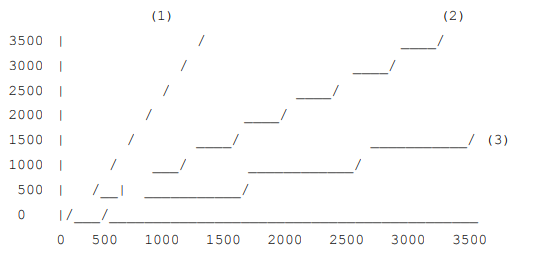
\includegraphics[width=0.8\textwidth]{images/scheduling.png}
    \caption{Отношение между виртуальным временем и настоящем временем в зависимости от приоритета. X - wall-time clock, Y - virtual clock. (1) - nice +5, (2) - nice 0, (3) - nice -5}
    \label{fig:mesh1}
\end{figure}

\pagebreak
Имея такую структуру, можно за $O(log N)$ выбирать следующую задачу:
\begin{lstlisting}
struct sched_entity *__pick_first_entity(struct cfs_rq *cfs_rq)
{
 struct rb_node *left = cfs_rq->rb_leftmost;
 if (!left)
    return NULL;
 return rb_entry(left, struct sched_entity, run_node);
}
\end{lstlisting}
\end{document}


